% Created 2022-04-08 ven. 22:40
% Intended LaTeX compiler: pdflatex
\documentclass[11pt]{article}
\usepackage[utf8]{inputenc}
\usepackage[T1]{fontenc}
\usepackage{graphicx}
\usepackage{grffile}
\usepackage{longtable}
\usepackage{wrapfig}
\usepackage{rotating}
\usepackage[normalem]{ulem}
\usepackage{amsmath}
\usepackage{textcomp}
\usepackage{amssymb}
\usepackage{capt-of}
\usepackage{hyperref}
\usepackage{lmodern} % Ensures we have the right font
\usepackage{graphicx}
\usepackage{amsmath, amsthm, amssymb}
\usepackage[table, xcdraw]{xcolor}
\usepackage{fancyhdr}
\fboxsep=0mm
\fboxrule=1pt
\usepackage{letltxmacro}
\LetLtxMacro\latexincludegraphics\includegraphics % save the function
\renewcommand{\includegraphics}[2][]{\fcolorbox{black}{white}{\latexincludegraphics[#1]{#2}}}
\usepackage[left=2cm,right=2cm,top=3cm,bottom=3cm]{geometry}
\pagestyle{fancy}
\fancyhf{}
\lhead{Modify in current org file : \lhead{foo}}
\rfoot{Page \thepage}
\usepackage{titling}
\setlength{\droptitle}{-8ex}
\pretitle{\begin{flushleft}\Large\bfseries}
\posttitle{\par\end{flushleft}}
\preauthor{\begin{flushleft}\large}
\postauthor{\end{flushleft}}
\predate{\begin{flushleft}}
\postdate{\end{flushleft}}
\usepackage[normalem]{ulem}
\usepackage{sectsty}
\sectionfont{\underline}
\makeatletter
\def\@seccntformat#1{%
\expandafter\ifx\csname c@#1\endcsname\c@section\else
\csname the#1\endcsname\quad
\fi}
\makeatother
\definecolor{bblue}{HTML}{275382}
\usepackage[colorlinks]{hyperref}
\hypersetup{colorlinks, linkcolor=bblue, urlcolor=bblue}
\usepackage[font={color=gray},figurename=Fig.,labelfont={it}]{caption}
\usepackage{graphicx}
\setkeys{Gin}{width=0.8\linewidth}
\setkeys{Gin}{height=0.7\textheight}
\setkeys{Gin}{keepaspectratio}
\usepackage{enumitem}
\setlist{noitemsep}
\renewcommand{\contentsname}{Sommaire}
\usepackage{listings}
\usepackage{xcolor}
\usepackage[utf8]{inputenc}
\usepackage[table]{color}
\definecolor{grayW}{rgb}{0.94,0.94,1.00}
\definecolor{bluegr}{rgb}{0.0,0.50,0.50}
\definecolor{redp}{rgb}{0.80,0.10,0.10}
\lstset{
backgroundcolor=\color{grayW},
keywordstyle=\color{bluegr},
stringstyle=\color{redp},
basicstyle=\ttfamily\scriptsize,
breakatwhitespace=false,
numbers=left,
numbersep=5pt,
}
\lhead{DUREL Enzo, VILLEPREUX Thibault}
\rhead{POO - Puissance 4}
\author{DUREL Enzo, VILLEPREUX Thibault}
\date{\today}
\title{Projet - Puissance 4 - Java}
\hypersetup{
 pdfauthor={DUREL Enzo, VILLEPREUX Thibault},
 pdftitle={Projet - Puissance 4 - Java},
 pdfkeywords={},
 pdfsubject={},
 pdfcreator={Emacs 27.1 (Org mode 9.3)}, 
 pdflang={English}}
\begin{document}

\maketitle
\tableofcontents

\thispagestyle{fancy}

\newpage

\section{Introduction}
\label{sec:orgd1a5943}

\subsection{Compilation}
\label{sec:orgdb57576}

Lancez le Makefile avec la commande \texttt{make} dans le dossier \texttt{cd projet-java}.\\

\subsection{Exécution}
\label{sec:orga77af6e}

Exécuter le script bash \textbf{exec} qui lance le programme \textbf{Main} dans le dossier\\
\textbf{projet-java/build}.\\

Si une erreur survient lors du programme, elle est écrite dans le fichier \textbf{log.txt}.\\

\subsection{Puissance 4}
\label{sec:org7c6623c}

Le principe est simple : insérer un pion chacun son tour dans la grille verticale. Le\\
gagnant est le premier à avoir aligné 4 pions de la même couleur, horizontalement,\\
verticalement, ou en diagonale. Tout l'enjeu de la partie réside dans la stratégie\\
adoptée pour mettre l'adversaire en échec.\\


\newpage

\section{UML du Puissance 4}
\label{sec:org0249ede}

\begin{figure}[htbp]
\centering
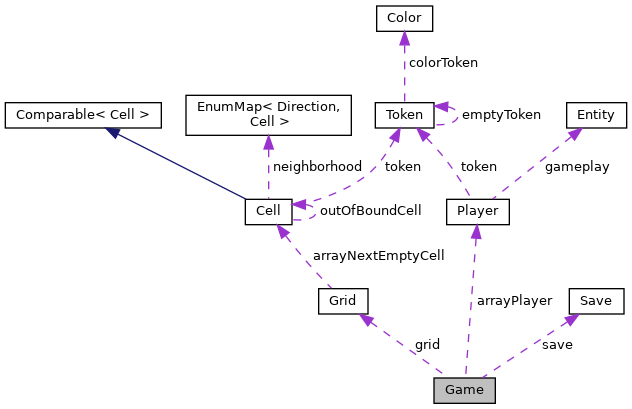
\includegraphics[width=.9\linewidth]{../doc/html/class_game__coll__graph.png}
\caption{UML du Puissance 4}
\end{figure}

\section{Explication de code}
\label{sec:org14eca12}

\subsection{Introduction}
\label{sec:org84bb9f7}

La documentation étant entièrement disponible, nous allons nous attarder uniquement sur\\
les principales classes de notre logiciel ainsi que leur fonctionnement global.\\

Pour cela nous nous appuirons sur le diagramme de la classe ainsi que certaines\\
fonctions jugées principales qui sont expliquées avec leurs \hyperref[org58a15d4]{graphes respectifs}.\\

\subsection{Classe Cell\label{orgc81d8e8}}
\label{sec:org7ab91b8}

Nous allons maintenant présenter la classe qui représente \textbf{le plateau de jeu} du\\
puissance 4. Il s'agit de \texttt{public class Cell}.\\

\subsubsection{Attributs}
\label{sec:orgd992ba5}

Nous avons redéfini la cellule \texttt{null}, celle-ci s'appelle outOfBoundCell et est\\
renvoyé lorsque qu'on accès à une cellule qui n'existe pas. Nous avons rédéfini car\\
plus compréhensible sémantiquement et pour éviter d'avoir des null qui se promène dans\\
notre code. Cet attribut est statique donc toujours de même référence.\\

Chaque cellule possède un jeton (Token) qui est ici juste un objet possédant une\\
certaine couleur (\hyperref[org4fc9396]{Color}).\\

Chaque cellule possède aussi 4 voisins directes (\textbf{UP}, \textbf{DOWN}, \textbf{RIGHT}, \textbf{LEFT})\\
représenté ici par une EnumMap où les clés sont une direction (\hyperref[org010dbac]{Direction}) donnée et\\
les valeurs la référence à sa cellule voisine dans la direction.\\

\subsubsection{Méthodes}
\label{sec:org38f0060}

\begin{enumerate}
\item \texttt{setNeighbor: Cell*Direction -> ()} \label{org45c9cd6}
\label{sec:org76b1234}

Cette méthode prend en paramètre une cellule (\hyperref[orgc81d8e8]{Cell}) et une direction (\hyperref[org010dbac]{Direction}) où\\
la cellule représente la cellule voisine a attribue dans la direction par rapport à\\
la cellule dont la méthode est appelée.\\

Elle actualise l'EnumMap représentant les voisins d'une cellule dont la clé est la\\
direction donnée. La cellule doit être non \texttt{null}, la direction doit être non \texttt{null}.\\

\item \texttt{getNeighbor: Direction -> Cell} \label{org48fb67a}
\label{sec:orga799806}

Cette méthode prend en paramètre une direction (\hyperref[org010dbac]{Direction}) et renvoie la cellule\\
voisine dans la direction de la cellule qui appelle la méthode.\\

Dans le cas où la cellule voisine est null, la cellule invalide outOfBoundCell est\\
renvoyée. La direction doit être non nulle.\\

\item \texttt{check: () -> boolean}
\label{sec:orgb9fea08}

La fonction check vérifie si la cellule qui appelle la méthode satisfait les\\
conditions d'arrêt du jeu: ici si 4 jeton (Token) de suite, sont de la même couleur\\
et aligné suivant la même direction.\\

Donc nous vérifions pour chaque direction possible acceptés si le nombre dans la\\
direction donnée de jetons de la même couleurs est supérieur ou égal à 4.\\

Pour cela nous utilisons deux méhodes définies en surcharges.\\

La première ne prend en paramètre qu'une seule direction et compte suivant les\\
directions des cellules voisines directes (\textbf{UP}, \textbf{DOWN}, \textbf{RIGHT}, \textbf{LEFT})\\

La deuxième prend en paramètre deux directions qui définiront le comptage en\\
diagonale. En effet, une diagonale n'est juste composé de 2 directions primitives.\\

Les diagonales sont récupérées dans l'Enum (\hyperref[org010dbac]{Direction}) par la méthode \texttt{getDiagonales}\\
et sont renvoyé sous la forme d'une EnumMap où les clés sont les directions\\
primitives et les valeurs une direction associée formant une diagonales. Les\\
diagonales renvoyées sont uniques.\\

Le nombre de voisin est définit par la somme des même cellules à partir de la cellule\\
courante dans la direction donnée et dans sa direction opposé qui est récupéré grâce\\
à la fonction \texttt{getOpposite} dans l'Enum (\hyperref[org010dbac]{Direction}).\\

\begin{enumerate}
\item \texttt{numberOfSameNeighbor: Direction -> int}
\label{sec:org2c5c48f}

Cette méthode prend en paramètre une direction et compte dans cette direction et à\\
partir de la cellule le nombre de jetons similaires.\\

Elle utilise pour cela la récursivité. Le cas d'arrêt est : Si la prochaine cellule\\
est la cellule invale outOfBoundCell ou que le jeton de la cellule n'est plus le\\
même que la cellule précédente. Sinon, elle renvoie 1 + appel de cette méthode sur\\
la cellule suivant dans la direction donnée.\\

\item \texttt{numberOfSameNeighbor: Direction*Direction -> int}
\label{sec:orgcd9ad29}

Cette méthode est similaire à la précédente, la prochaine cellule est la cellule\\
suivant les deux directions données. La condition d'arrêt est la même, l'appel\\
récursif est le même.\\
\end{enumerate}
\end{enumerate}

\subsection{Classe Grid\label{orgbab96b7}}
\label{sec:org8a51e52}

Nous allons maintenant présenter la classe qui représente \textbf{le plateau de jeu} du\\
puissance 4. Il s'agit de \texttt{public class Grid}.\\

\subsubsection{Attributs}
\label{sec:org3067227}

La classe \hyperref[orgbab96b7]{Grid} est composé d'un tableau de cellules (\hyperref[orgc81d8e8]{Cell}) contenant les prochaines\\
cellules vides de chaque colonnes. Lorsque la colonne est pleine, la prochaine cellule\\
vide est la cellule située la plus haute dans la grille.\\

Nous avons utilisée cette représentation parce que sémantiquement nous n'avions besoin\\
que de savoir cela pour permettre au joueur de jouer. De plus nous avons donc un gain\\
de mémoire.\\

La classe comporte également deux attributs static représentant respectivement la\\
largeur \textbf{WIDTH} et la hauteur \textbf{HEIGHT}.\\

\subsubsection{Méthodes}
\label{sec:org239e0e6}

Nous allons vous présenter maintenant quelques fonctions principales de cette classe.\\

\begin{enumerate}
\item \texttt{initGrid: () -> ()}
\label{sec:org1872e4e}

Voici la fonction d'initialisation de la grille. Elle crée un tableau 2D de cellules\\
(\hyperref[orgc81d8e8]{Cell}), elle assigne à chaque cellule leurs voisins respectifs (\textbf{UP}, \textbf{DOWN},\\
\textbf{RIGHT}, \textbf{LEFT}) grâce à la fonction \hyperref[org45c9cd6]{setNeighbor: Cell * Direciton ->()} de (\hyperref[orgc81d8e8]{Cell}).\\

Nous remplissons ensuite le tableau des prochaines cellules vides définis précédement\\
en prenant comme première cellule la cellule situé la plus en bas de chaque colonnes\\
(car grille initialisé à vide).\\

\item \texttt{getNextEmptyCellAt: int -> ()}
\label{sec:orgaed8be9}
\item \texttt{UpToNextEmptyCellAt: int -> ()}
\label{sec:org7c2e71b}
\item \texttt{loadGrid: String*Token[] -> ()}
\label{sec:org734e89b}
\end{enumerate}

\subsection{Classe Player\label{org9fe4881}}
\label{sec:orgd262621}
\subsubsection{Attributs}
\label{sec:org7365c36}
\subsubsection{Méthodes}
\label{sec:orgd5c4bd7}
\begin{enumerate}
\item \texttt{initToken: int -> Token}
\label{sec:org88d0e0d}
\end{enumerate}
\subsection{Classe Game\label{org0efadc8}}
\label{sec:orge4690e1}
\subsubsection{Attributs}
\label{sec:org4a8c3b9}

\subsubsection{Méthodes}
\label{sec:orgcd22710}
\begin{enumerate}
\item \texttt{loadSave: String -> ()}
\label{sec:org29bccb2}
\item \texttt{play: () -> ()}
\label{sec:org41f9772}
\item \texttt{chooseAColumn: () -> int}
\label{sec:org9747597}
\item \texttt{playAToken: Token*int -> boolean}
\label{sec:orgd875b91}
\item \texttt{isEnd: () -> ()}
\label{sec:orgdadc643}
\begin{enumerate}
\item \texttt{hasWin(): () -> boolean}
\label{sec:orgf6d1993}
\item \texttt{isTie: () -> boolean}
\label{sec:orgadea1d0}
\end{enumerate}
\end{enumerate}

\subsection{Classe Save\label{org7fda068}}
\label{sec:org54c34f3}
\subsubsection{Attribut}
\label{sec:org397adc2}
\subsubsection{Méthodes}
\label{sec:org6c1a313}
\begin{enumerate}
\item write: Object -> ()
\label{sec:org81ef721}
\item read: () -> String
\label{sec:org5715191}
\end{enumerate}
\subsection{Enumérations}
\label{sec:orge99671c}
\subsubsection{Color\label{org4fc9396}}
\label{sec:org13ed5b2}
\subsubsection{Direction\label{org010dbac}}
\label{sec:orga11bd23}
\section{Documentation\label{org58a15d4}}
\label{sec:orgf28efab}

La documentation est entièrement disponible dans le dossier \textbf{doc/}. La documentation a\\
été générer grâce à l'outil DOxyGen (1.9.3). Elle contient le diagramme de classe de\\
chaque classe du logiciel ainsi que les graphes d'appels (Call \& Caller).\\

La documentation est mise sous \textbf{HTML} et \textbf{\LaTeX{}}.\\

Le fichier \textbf{HTML} est disponible \href{/home/hozen/cur/projet-java/doc/html/index.html}{../doc/html/index.html}.\\

Le fichier \textbf{PDF} compilé à partir du \textbf{\LaTeX{}} est disponible \href{/home/hozen/cur/projet-java/doc/latex/refman.pdf}{../doc/latex/refman.pdf}.\\

\section{Git\label{org580b1c4}}
\label{sec:orgd9b32ea}

Le projet est disponible et hébergé sur le \href{https://gitlab.isima.fr}{GitLab de l'ISIMA}\\

\newpage
\listoffigures
\end{document}
